\section{3D Finger Knuckle of 3D Finger Knuckle Database}

I have use the matlab code that offered by the FKNet to generate the 3D finger knuckle images for getting the depth information. But it is different that the input image size. The FKNet will resize the original image size $148*212$ to $70*100$ as the testing dataset, and crop from the $70*100$ to $48*80$ as the training dataset. As for RFNet, I just use the original image as the input data. Then the experiment protocol will generate $190*6$ genuine matching scores, and $190*189*6$ imposter matching scores. From the experiment result, we can get that the RFNet is the best model for the 3D Finger Knuckle Database.

\begin{figure}[H]
    \centering
    \begin{subfigure}[b]{0.8\linewidth}
        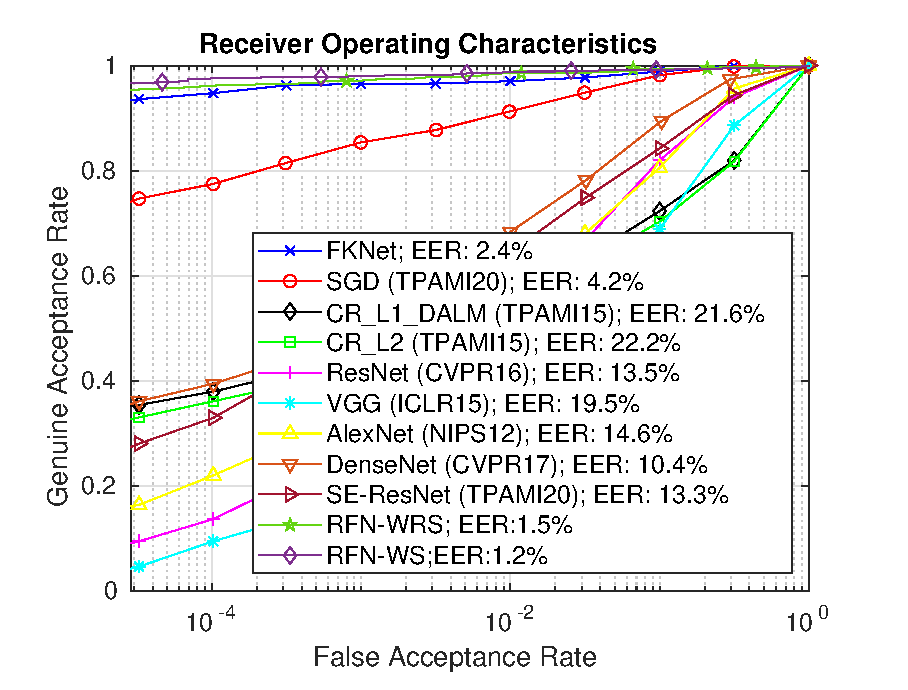
\includegraphics[width=\linewidth]{Figures/fknet/3d1s3d-roc_compare_new.eps}
    \end{subfigure}
\end{figure}